\documentclass{lib/wa}

\begin{document}

\maketitle{Jan von Bargen}{Informatik}
  {Joschka Kintscher}{Digitale Medien}
  {Janine Thönsing}{Digitale Medien}{24.10.2013}{1}

% ------------------------------------------------------------------------------
% Aufgabe A
% ------------------------------------------------------------------------------

\section{Quellensuche}

  \begin{enumerate}
    \item\textbf{new media \& society}
    \newline
    Standort: Zentrale/E4, Regal: z puz, Buch: jc/313
    \newline
    \cite{vergeer2013}

    \item\textbf{Wirtschaftsinformatik 3/2006}
    \newline
    Standort: Zentrale/E2, Regal: z kyb, Buch: 400 j/962
    \newline
    \cite{thiesse2006}

    \item\textbf{Informatik-Spektrum}
    \newline
    \cite{lintu2009}

    \item\textbf{FIfF Kommunikation}
    \newline
    \cite{bockerman2013}

    \item\textbf{Lecture Notes in CS}
    \newline
    \cite{temdee2006}

    \item\textbf{Film über Joseph Weizenbaum}
    \newline
    Standort: Zentrale/E4 Mediathek, Film: ph0858
    \newline
    \cite{haas2006}
    \newline
  \end{enumerate}

% ------------------------------------------------------------------------------
% Aufgabe B
% ------------------------------------------------------------------------------

\newpage

\section{LaTeX}

  Das Buch "LaTeX: Basissystem, Layout, Formelsatz" \cite{braune2006} liefert viele Programmierbeispiele, die durchweg anschaulich mit Screenshots illustriert und von farblich formatierten Syntaxbeispielen begleitet werden. Der Inhalt folgt einer sehr klaren und einfach zu verstehenden Struktur. Anders als viele andere Fachliteratur ist das gesamte Werk in deutscher Sprache veröffentlicht und macht es so vielen Einsteigern deutlich einfacher. Andere Einführungsbücher, wie z.B. "Latex Band 1: Einführung" machen deutlich weniger Syntax- und Anwendungsbeispiele und erlauben es auf Grund ihres sehr technischen Aufbaus weniger, einen einfachen Einstieg in die Thematik zu finden.
  \newline

% ------------------------------------------------------------------------------
% Aufgabe C
% ------------------------------------------------------------------------------

\section{Kurz-Betrachtung}

  Auf Grund des Open Source Charakters von Wikipedia ist es oftmals schwierig, den genauen Urheber einer Aussage bzw. eines Artikels ausfindig zu machen \cite{waters2007}.
  Da man also die Qualität eines Eintrages selten am Autor festmachen kann, spielen bei der Evaluation haeufig andere, jedoch gleichzeitig irreführende Faktoren, wie z.B. die Verwendung von Medien, eine Rolle. \cite{lucassen2010}.
  Durch den sehr hohen Suchrank einzelner Artikel bei Google landen viele Leser meist doch bei Wikipedia \cite{waters2007}.

  Aus unserer Praxiserfahrung heraus kommen wir zu dem Schluss, dass Wikipedia als direkte, wissenschaftliche Quelle nicht geeignet ist. Allerdings bietet Wikpiedia einen guten Einstiegspunkt in die weiterfuehrende Recherche und dient als Ueberblick ueber ein noch unbekanntes Thema.
  \newline

% ------------------------------------------------------------------------------
% Aufgabe D
% ------------------------------------------------------------------------------

\section{Gliederung eines Referats}

  \subsection*{Gliederung}
    \begin{description}[style=nextline]
      \item[Einstieg: Aktuelles Thema]
      Neuste Plagiatsvorwürfe gegen Steinmeier

      \item[Wer plagiiert und warum?]
      Unterschiedliche Gruende zu kopieren und keine richtigen Quellenangaben zu machen

      \item[Was ist ein Plagiat?]
      Definition und Rechtslage

      \item[Ist die Menschheit bereit für ein Überangebot von Informationen?]
      Durch das Internet hat jeder Mensch Zugriff auf fast alle Informationen, was neue Verantwortungen mit sich bringt

      \item[Meinungen zu Urheberrecht und geistiges Eigentum]
      Darstellung verschiedener Sichtweisen zum Thema Lizenzen

      \item[Wie arbeite ich richtig mit verschiedenen Quellenarten?]
      Korrektes wissenschaftliches Arbeiten mit Quellen und Verweisen
    \end{description}

  \subsection*{Quellen}
    \begin{enumerate}
      \item[\cite{greiner2013}]
        Die unterschiedlichen Plagiatstypen und rechlichte Konsequenzen werden übersichtlich in verschiedenen Kontexten dargestellt.

      \item[\cite{wulff2008}]
        Der Artikel verbindet allgemeine Informationen zum Thema Plagiate mit Sachinformationen und Studien und beschreibt verschiedene Wege des Umgangs mit geistigem Eigentum im Internetzeitalter.

      \item[\cite{schad2008}]
        Sehr deutlicher Kommentar zum Thema Plagiate und der Veroeffentlichung wissenschaftlicher Arbeiten im Internet.
    \end{enumerate}

% ------------------------------------------------------------------------------
% Aufgabe E
% ------------------------------------------------------------------------------

\section{Strukturieren}

  \begin{figure}[ht]
    \centering
    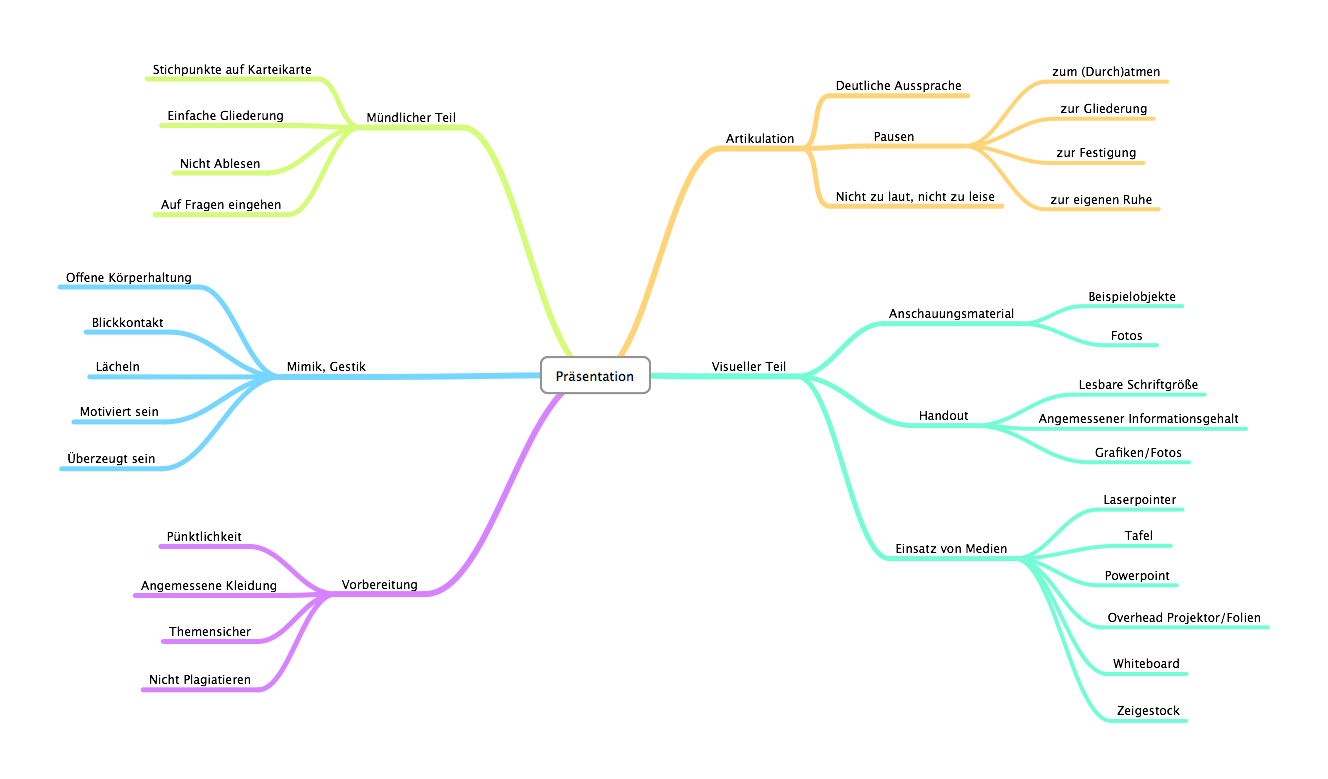
\includegraphics[width=\textwidth]{assets/praesentation.png}
    \caption{Wichtige Aspekte bei der Vorbereitung und Gestaltung eines Vortrages}
  \end{figure}

% ------------------------------------------------------------------------------
% Literaturverzeichnis
% ------------------------------------------------------------------------------

\newpage

\bibliography{lib/literaturverzeichnis}
\bibliographystyle{alpha}

\end{document}
